\chapter{ミリ波観測のデータ解析}
\label{ch:mm_analysis}
\ref{ch:mm_obs}章で述べたように、トロムソは我々にとっては観測自体が初めての場所であり、昭和基地においては分光計を更新してから初めての観測である。
そのため、それぞれ観測装置の立ち上げ後に行われたテスト観測のデータを1つずつ精査した。
本章では、その手法と結果について述べる。\par

\ref{ssec:obs_syowa}節の図\ref{fig:NO_spectr}で示したように、\ce{NO}の輝線スペクトルはとても微弱である。
そのため、物理量の算出に十分なS/N比となるようにデータを処理し、輝線スペクトルを得る必要がある。
そこで今回は、全体のデータから設定した特定の条件をクリアした解析に用いることができるデータのみを選別する「スクリーニング」と、下層大気や観測装置の特性に起因する受信電波強度の補正を行った。
ミリ波分光計の観測システムは市販されているものではないため、ほぼ全てのハードウェア・ソフトウェアは自作となっており、今回用いるスクリーニングおよび電波強度の補正に必要なプログラムは自ら作成した。\par

スクリーニングと電波強度の補正については、以下のようにそれぞれ2つの観点から行った。
\begin{itemize}
    \item データのスクリーニング
    \begin{itemize}
        \item 光学的厚みの測定データを基にしたスクリーニング(\ref{sec:screening_opticaldepth}節)
        \item NOスペクトルデータのバックグラウンドノイズを基にしたスクリーニング(\ref{sec:screening_spectralnoise}節)
    \end{itemize}
    \item 電波強度の補正
    \begin{itemize}
        \item 下層大気の光学的厚みの影響の補正(\ref{sec:correction_opticaldepth}節)
        \item NOスペクトルデータのベースラインの補正(\ref{sec:correction_baselinefitting}節)
    \end{itemize}
\end{itemize} \par
本研究における解析を行うにあたって、トロムソでは2018年12月26日〜2019年3月10日の期間に行われたテスト観測のデータを用い、昭和基地では2023年3月22日〜2023年3月30日の観測データを用いた。
これらのスクリーニングを行った結果、本研究で用いたデータの解析期間はトロムソでは2019年1月23日〜2019年2月4日と2019年2月17日〜2019年2月20日、南極・昭和基地では2023年3月22日〜2023年3月30日となった。
両極域での比較という観点では、トロムソ・昭和基地両方において同時期の観測データを用いるのが望ましい。
しかしながら、トロムソにおいて\today 時点で使用可能なデータは今回用いる期間のもののみであり、この時期における昭和基地は観測条件が悪く、解析に用いることができるデータを得ることができなかった。
そのため、今回は異なる時期での解析を行ったことに注意してほしい。
以下では、それぞれの解析手法とその結果について順番に述べて、\ref{sec:derive_columndensity}節は\ce{NO}の柱密度の導出について述べる。


\section{光学的厚みの測定データを基にしたスクリーニング}
\label{sec:screening_opticaldepth}
\ref{ssec:obs_opticaldepth}節で述べたように、ミリ波分光計を用いた中層大気(主に上部成層圏〜下部熱圏)の地上観測では、下層大気(主に対流圏)による影響を受けるため、観測中定期的に実測する光学的厚みの測定データを用いて、この影響を取り除いている。
光学的厚みの測定を行っている間に大気分子の観測を行っているため、光学的厚みは大気分子の観測を行っている間、安定しているという前提の上で光学的厚みによる電波強度の補正を行っている。
従って、光学的厚みの測定データは観測データに対して充分に安定していなければならない。\par

図\ref{fig:optical_depth_tromsoe}に示しているデータは、トロムソの観測装置立ち上げ後に行われたテスト観測の期間に測定された光学的厚みの時間変化を表したものである。
\begin{figure}[htbp]
    \centering
    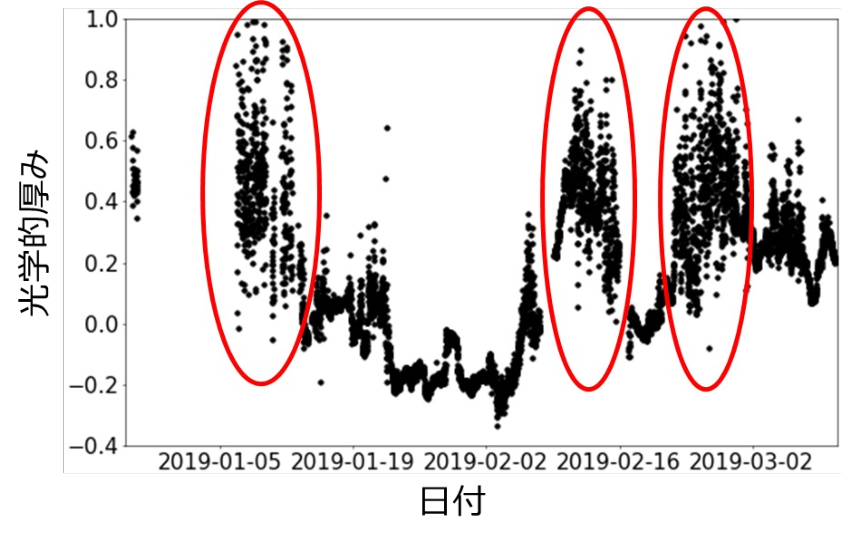
\includegraphics[width=\linewidth]{master_thesis_contents/master_thesis_fig/optical_depth_tromsoe.pdf}
    \caption{トロムソでの光学的厚み測定データの時間変化(~\cite{goto2021bachelor}より引用)}
    \label{fig:optical_depth_tromsoe}
\end{figure}
比較的値が安定している時期と、値が大きくばらついて安定していない時期がある(例として赤丸で示す)。
この赤丸で示された時期は、光学的厚みの典型値(たとえば南極昭和基地ではおよそ$0.1-0.4$の範囲の値をとる)とは大きく外れている。
% 何に基づく典型値でしょうか?先行研究で示されているものであれば、それを引用。
このように短時間で値の変動が大きい場合は、光学的厚みが測定される時間スケール(測定間隔はおよそ$12-13$分)で、下層大気の影響が変化しており一様でないことを表している。
そのため、離散的に測定された光学的厚みの値を用いて、その間に観測されたスペクトルデータの電波強度を一様に補正するには適さないと考えられる。\par

そこでまず、観測データの強度の補正に使用できる光学的厚みのデータを決定するために、光学的厚みの測定したデータそれ自体のスクリーニングを行うことを考えた。
このスクリーニングで残った期間の観測データを後の解析に用いることとする。\par

スクリーニング方法としては、まず1日ごとにデータを区切り
% (一日の間で測定される光学的厚みのデータ数は**個程度になる)
、それぞれの日でこれらの分散を計算し、その分散が$0.005$以下の値の日をとるデータを使用することとした。
分散の閾値を0.005としたのは、図\ref{fig:optical_depth_tromsoe}のデータを目視し、値が安定していると判断した2019年1月23日〜2019年2月4日の分散がいずれも0.005以下であったため、このように設定した~\cite{goto2021bachelor}。
この条件を設定することで、光学的厚みの変動が大きい、すなわち下層大気の影響が過度に大きく、データの質が安定しない時間帯を除去することができる。
南極・昭和基地の解析においても同条件でスクリーニングを行った。
% この章は、既に本研究の結果を示す章なので、南極のデータも具体的に示す。


\section{NOスペクトルデータのバックグラウンドノイズを基にしたスクリーニング}
\label{sec:screening_spectralnoise}
次に、\ref{sec:screening_opticaldepth}節のスクリーニングで残った\ce{NO}スペクトルの観測データにおいて、解析に使うことのできない質の悪いデータをスクリーニングすることを考える。
トロムソの観測期間の全取得データを精査した結果、スペクトルデータに含まれる顕著なノイズ成分というのは、周波数的に非常に狭く強度の強いスパイク状のノイズと、全体に渡ってランダムな強いノイズの2種類があることがわかった~\cite{goto2021bachelor}。
そこで、これらのスパイク状のノイズと全体的なノイズをそれぞれ自動的に判別する条件を決めることで、図\ref{fig:raw_spectrum}(a)のような質の良いデータのみを抽出することを目指す。\par

まず、NOスペクトルが存在する周波数($250.435-250.817\ \mathrm{GHz}$)を含む分光計の$5000-10000$チャンネルの範囲のデータに対し、二次曲線をフィッティングした。
この周波数帯にランダムノイズがどれだけ含まれているか調べるために、この近似値に対する測定値の二乗平均誤差を計算する。
ここでは$5000-10000$チャンネルにおいてスペクトルデータの典型的なベースラインの形状が二次関数的であったため、二次近似を用いることにした(図\ref{fig:raw_spectrum}(a)の赤線)。
\begin{figure}[htbp]
    \centering
    \begin{minipage}{0.33\linewidth}
        \centering
        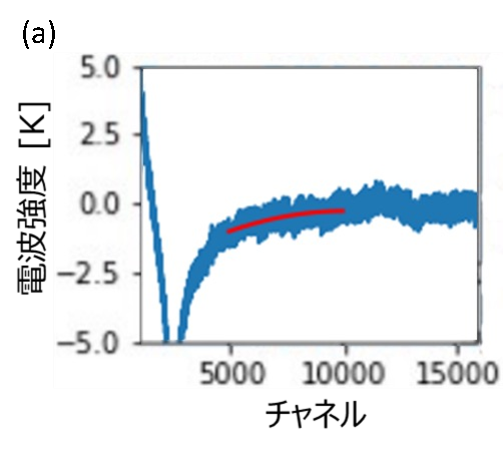
\includegraphics[width=\linewidth]{master_thesis_contents/master_thesis_fig/raw_spectrum_good.pdf}
    \end{minipage}
    \begin{minipage}{0.6\linewidth}
        \centering
        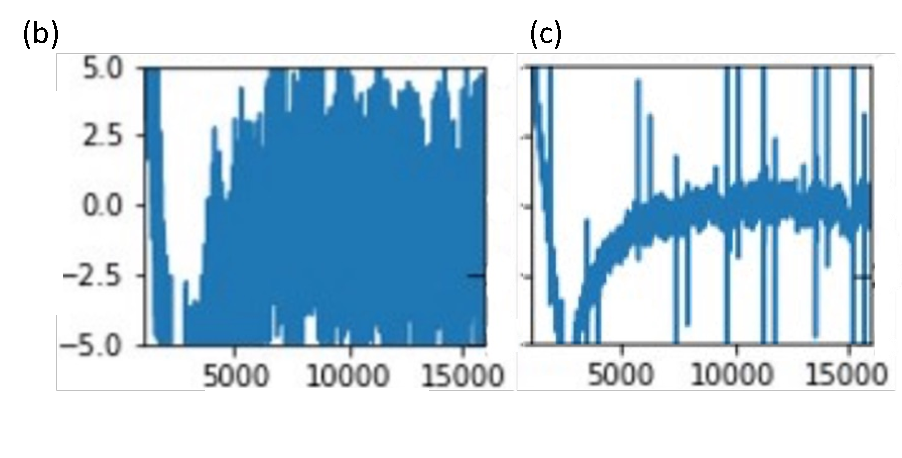
\includegraphics[scale=0.6]{master_thesis_contents/master_thesis_fig/raw_spectrum_bad.pdf}
    \end{minipage}
    \caption{(a) 解析に用いるために望ましい生データの一例($5000\, \mathrm{ch}$以下のデータは$239.093279\, \mathrm{GHz}$のオゾンの放射スペクトルデータがFRSWにより反映された結果、赤線は$5000-10000\, \mathrm{ch}$でのスペクトルデータの近似二次曲線を表す。)。(b)(c) スクリーニングしたいデータの例((b)は全体的にノイズを含む例、(c)はスパイク状のノイズを含む例を表す)。}
    \label{fig:raw_spectrum}
\end{figure}
この結果から、スクリーニング条件としては以下の2つを設定した~\cite{goto2021bachelor}。
\begin{itemize}
    \item 2乗平均誤差の整数丸め値が0ではない
    \item $5000-10000$チャンネルで強度の絶対値が$5\, \mathrm{K}$以上の値を含む
\end{itemize} \par
1つ目の条件は、全体的にノイズを含むデータ(たとえば図\ref{fig:raw_spectrum}(b))を判別・除去することを意図しており、2つ目の条件はスパイク状のノイズを含むデータ(たとえば図\ref{fig:raw_spectrum}(c))を除去することを意図している。
設定したスクリーニング条件が妥当かどうかの検証は、既に卒業研究~\cite{goto2021bachelor}にて行っている。
卒業結果では、明らかにノイズを含むデータについては意図した通りにスクリーニングをすることができており、質のよいデータのみを選ぶことに成功したという結論を得ている。
% このあとに節を追加し、南極昭和基地についても結果を述べる。


\section{トロムソにおける光学的厚みの測定データの異常値の検討}
\label{sec:correction_opticaldepth}
\ref{sec:screening_opticaldepth}節に述べたように、光学的厚みが短時間で変動している不安定なデータを除去したことによって、トロムソの観測データについては図\ref{fig:optical_depth_minus}のように期間A(2019年1月23日〜2019年2月4日)と期間B(2019年2月17日〜2019年2月20日)が残った。
しかし、期間Aにおいて光学的厚みが$-0.2$程度と負の値となっていることがわかった(図\ref{fig:optical_depth_minus}の赤丸)。
\begin{figure}[htbp]
    \centering
    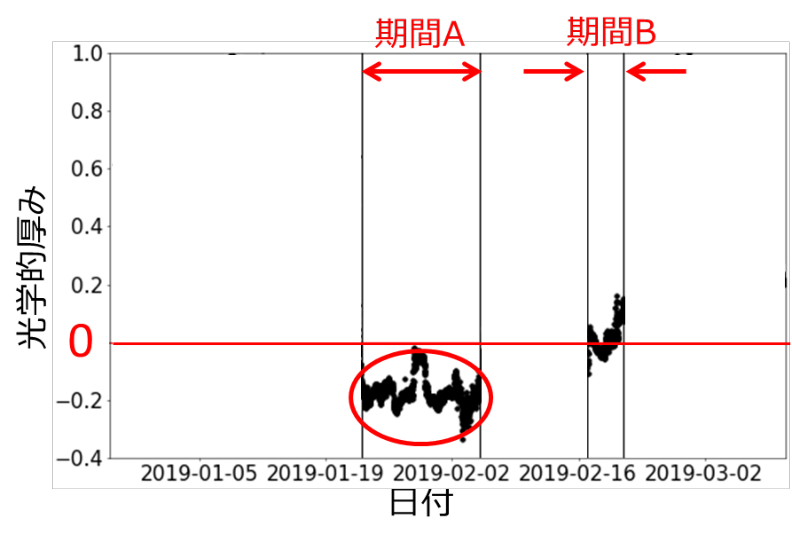
\includegraphics[width=\linewidth]{master_thesis_contents/master_thesis_fig/optical_depth_minus.pdf}
    \caption{トロムソにおいて負の値をとる光学的厚み(~\cite{goto2021bachelor}より引用)}
    \label{fig:optical_depth_minus}
\end{figure}
\ref{ch:mm_obs}章で述べた光学的厚みの算出方法のことを考えると、この値が負の値を取ることはない。
そこでこの原因を調べたところ、光学的厚みを算出する際に使用する式\eqref{eq:opticaldepth_plot}におけるプロットデータにおいて、各観測天頂角$z$における$\sec z$に対する$\ln \left( T_{obs\_ hot} - T_z \right)$が、もっとも観測天頂角が小さい($\sec z$が1番小さい)ところで異常に低くなっていた。
これによってフィッティングされた近似直線の傾きが正になってしまうことで、光学的厚みが負の値として計算されていることが分かった~\cite{goto2021bachelor}。
その模式図を図\ref{fig:optical_depth_slope_minus}、実際の測定データ例を図\ref{fig:optical_depth_measurement_good_bad}に示す。\par

\begin{figure}[htbp]
    \centering
    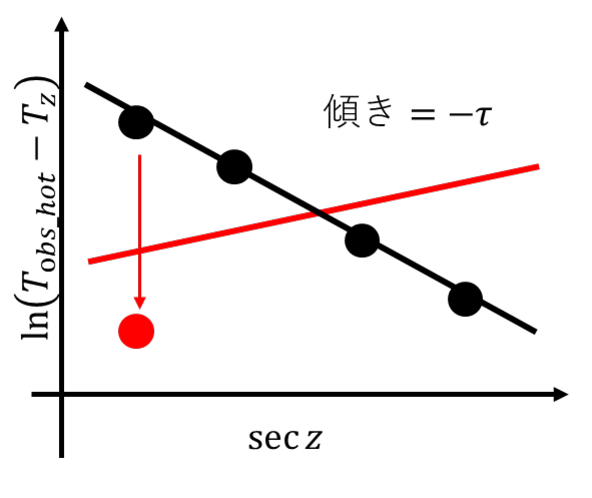
\includegraphics{master_thesis_contents/master_thesis_fig/optical_depth_slope_minus.pdf}
    \caption{プロットデータの落ち込みによる光学的厚みの計算値の変化(プロットデータの落ち込みにより近似直線が黒線→赤線に変わり、直線の傾きが変わる)~\cite{goto2021bachelor}より引用。}
    \label{fig:optical_depth_slope_minus}
\end{figure}
\begin{figure}[htbp]
    \centering
    \begin{minipage}{0.41\linewidth}
        \leftline{(a)}
        \centering
        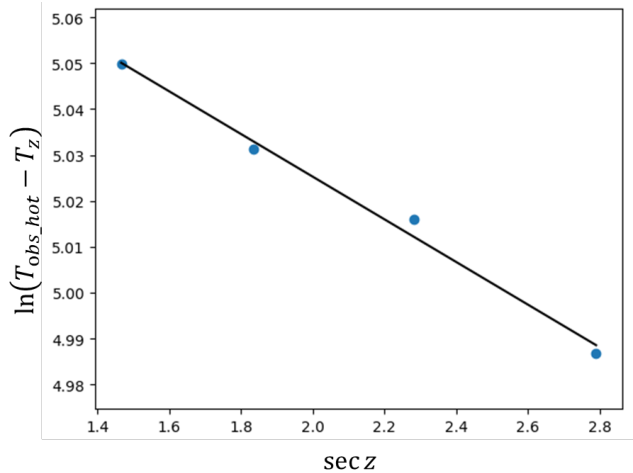
\includegraphics[width=\linewidth]{master_thesis_contents/master_thesis_fig/optical_depth_good.pdf}
    \end{minipage}
    \begin{minipage}{0.45\linewidth}
        \leftline{(b)}
        \centering
        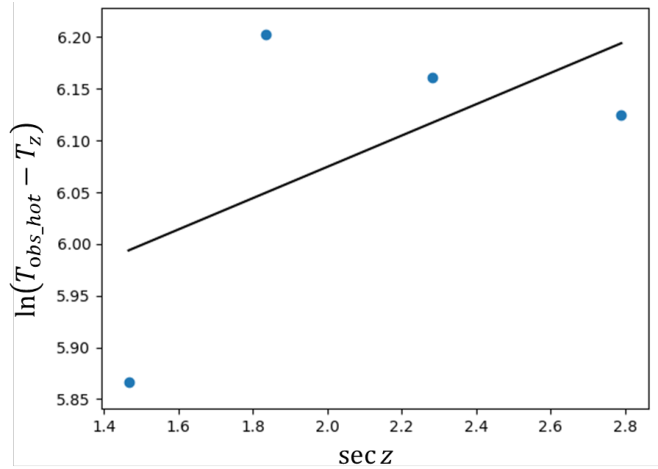
\includegraphics[scale=0.6]{master_thesis_contents/master_thesis_fig/optical_depth_bad.pdf}
    \end{minipage}
    \caption{(a) 望ましいプロットデータの一例(2019年2月17日5時51分頃測定)。(b) プロットデータが落ち込んだ実際のデータの一例。(2019年1月23日0時5分頃測定)。黒線は近似直線を表す。~\cite{goto2021bachelor}より引用。}
    \label{fig:optical_depth_measurement_good_bad}
\end{figure}
さらに、その天頂角が最も小さいデータの落ち込みの原因を調べたところ、この光学的厚みの値が負の値となっている期間の終わりごろに、光学的厚みの測定で用いる観測方向(\ref{ssec:obs_opticaldepth}節の表\ref{tb:secz_zdeg})にあるコンテナー側面の観測窓の上部に氷柱ができているのを見つけたという報告があり(図\ref{fig:icicles})、それが時期的に一致していることが分かった~\cite{goto2021bachelor}。
\begin{figure}[htbp]
    \centering
    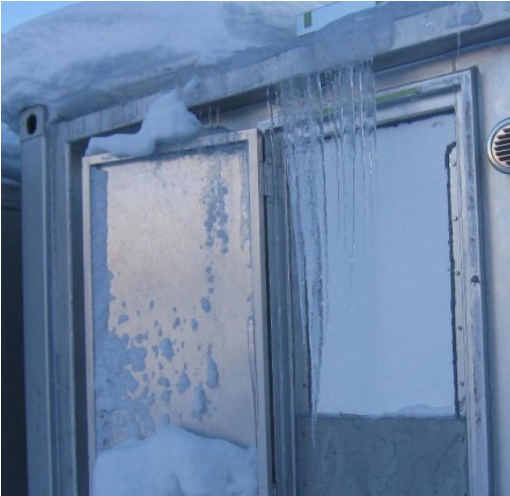
\includegraphics[width=\linewidth]{master_thesis_contents/master_thesis_fig/icicles.pdf}
    \caption{側窓にできた氷柱(~\cite{goto2021bachelor}より引用)}
    \label{fig:icicles}
\end{figure}
したがって、天頂角がもっとも小さい角度で測定された電波強度は、この氷柱の影響を受けてしまった可能性があると考えられる。
従ってこの期間は、天頂角のもっとも小さい方向の測定データは用いずに光学的厚みを算出することにした。
この妥当性の検証は卒業研究~\cite{goto2021bachelor}にて既に行っている。
卒業研究では、氷柱の影響を受けたとみられる期間において、光学的厚みの補正ができており、氷柱が除去された期間においては本来の値とほぼ一致しているため補正せずに用いることができるという結論を得ている。


\section{NOスペクトルデータのベースラインの補正}
\label{sec:correction_baselinefitting}
\ref{sec:screening_opticaldepth}節や\ref{sec:screening_spectralnoise}節によるスクリーニングで残った期間における\ce{NO}スペクトルデータについて、積分を行う。
昭和基地で行われた先行研究であるIsonoらによるデータ解析の結果~\cite{isono2014ground}より、24時間の積分をすることで十分なS/N比が得られることが示されている。
積分したスペクトルデータには、観測対象である\ce{NO}の輝線スペクトルだけでなく、下層大気や装置由来の連続波成分が含まれているため、ベースラインの補正を行う必要がある。
本研究では、\ce{NO}スペクトルから外れた両端におけるデータがバックグラウンドの成分を表していると考え、これをベースラインとして近似から求め、元のスペクトルから差し引くことにした。
これにより、FRSWで除去しきれなかったオフセット成分や周波数特性のうねりなどが除去され、観測対象の\ce{NO}スペクトルのみを取り出すことができる。\par

ベースラインの補正の模式図を図\ref{fig:baseline_correct_schema}に示す。
\begin{figure}[htbp]
    \centering
    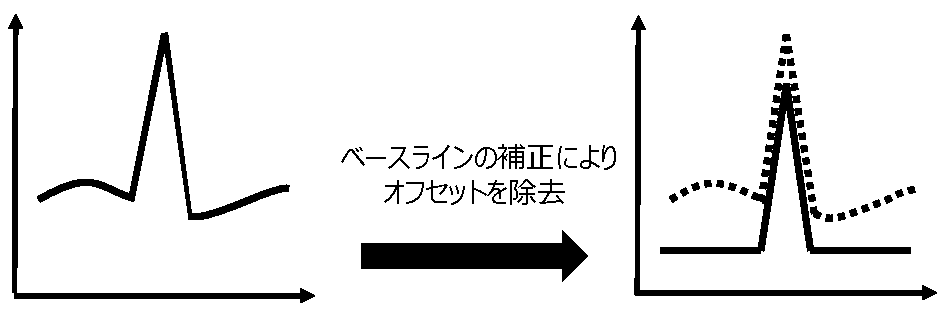
\includegraphics[width=\linewidth]{master_thesis_contents/master_thesis_fig/baseline_correct_schema.pdf}
    \caption{ベースライン近似を用いたベースラインの補正}
    \label{fig:baseline_correct_schema}
\end{figure}
ベースラインの近似に用いるデータは、図\ref{fig:baseline_range}の赤色で示した\ce{NO}スペクトルの両端のそれぞれ$5\, \mathrm{MHz}$の範囲を使用した。
この範囲は、対象とするNOの放射スペクトル成分が含まれないと考えられる。
\begin{figure}[htbp]
    \centering
    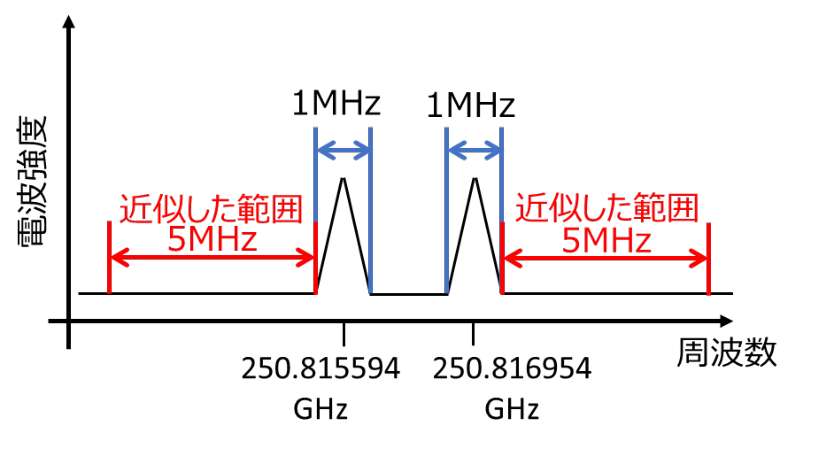
\includegraphics[width=\linewidth]{master_thesis_contents/master_thesis_fig/baseline_range.pdf}
    \caption{ベースラインを補正する元となる周波数の範囲(赤色で表示。青色は検出するスペクトルの幅を示している。例としてトロムソで用いた2本の輝線スペクトルの場合を示した。)}
    \label{fig:baseline_range}
\end{figure}
スペクトルデータを見ると、この周波数帯では典型的なベースラインの形状が、図\ref{fig:baseline_curve}に示す赤い曲線のような三次関数的な形であったので、ここでは三次関数で近似を行うことにした。
\begin{figure}[htbp]
    \centering
    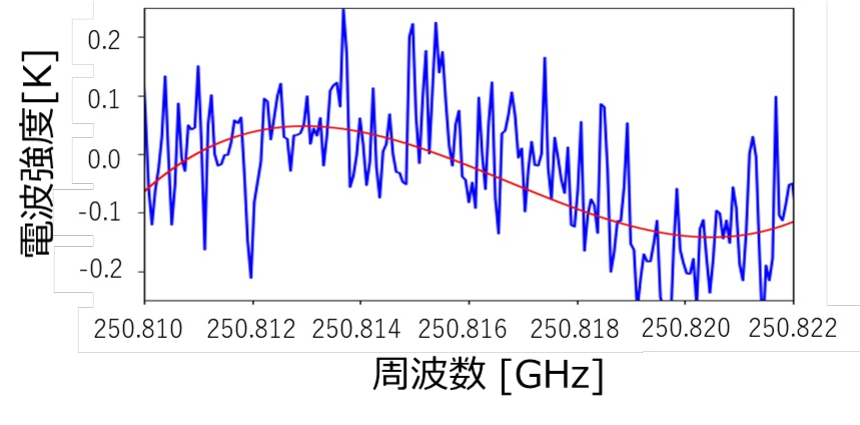
\includegraphics[width=\linewidth]{master_thesis_contents/master_thesis_fig/baseline_curve.pdf}
    \caption{三次関数的な形のベースライン(~\cite{goto2021bachelor}より引用)}
    \label{fig:baseline_curve}
\end{figure}
また、\ce{NO}の各スペクトル幅は$1\, \mathrm{MHz}$と仮定した。
このように仮定したのは対象の時期の日ごとのデータにおいて、放射スペクトルの幅の大きさがどの日のデータにおいてもおよそ$1\, \mathrm{MHz}$であることが確認できたためである(図\ref{fig:no_spectr_exp}にあるデータの一例においても、\ce{NO}スペクトル根本での幅がおよそ$1\, \mathrm{MHz}$であることが確認できる)。
% このあと、南極のデータについても説明
\begin{figure}[htbp]
    \centering
    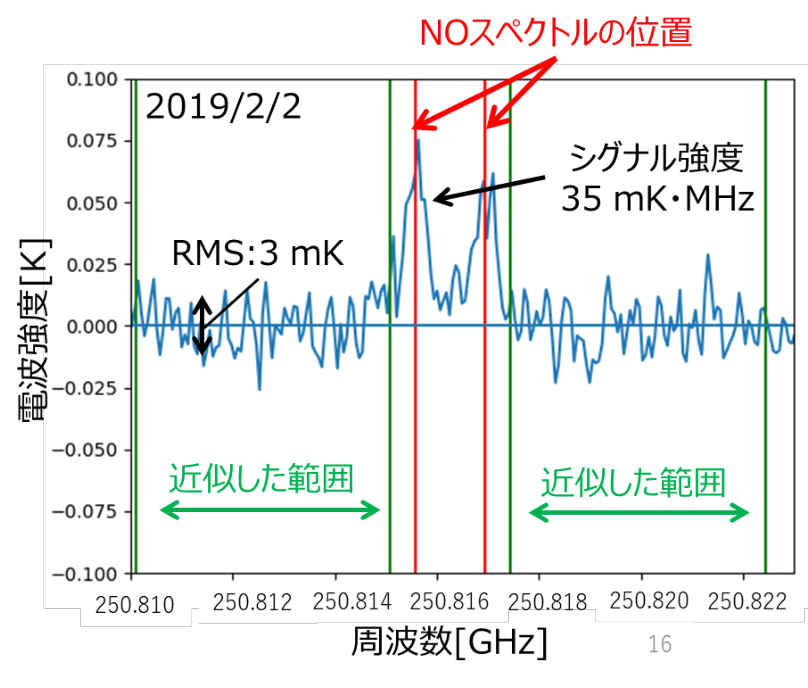
\includegraphics[width=\linewidth]{master_thesis_contents/master_thesis_fig/no_spectr_exp.pdf}
    \caption{スペクトルの検出の一例。2019年2月2日おける24時間積分によるスペクトルデータの一例。赤線は検出するスペクトルがある周波数の位置、緑線はベースライン近似に用いたスペクトルデータの範囲を示す。赤線と一番近くにある緑線の間が輝線スペクトルピークから端の間($=0.5\ \mathrm{MHz}$)にあたる。シグナル強度とRMSについては柱密度の導出(\ref{sec:derive_columndensity}節)で用いる(~\cite{goto2021bachelor}より引用)}
    \label{fig:no_spectr_exp}
\end{figure}
\clearpage


\section{NO柱密度(Column Density)の導出}
\label{sec:derive_columndensity}
柱密度とは高度方向に密度を足し合わせたものであり、
今回はスペクトルの線形から$70\, \mathrm{km}$以上に存在する\ce{NO}分子についてみたものとなる。
% これの理由が不明確ですので、説明をすること。
まず、本研究で用いたそれぞれの輝線スペクトルにおいて柱密度の導出を行った。
柱密度の導出方法は、先行研究~\cite{isono2014ground}を参考にして行った。
導出に用いた式は以下である。
\begin{gather}
    N_{\mathrm{NO}} = A \times T_{\mathrm{atm}} \times \int T_{\mathrm{NO}}d\nu
    \label{eq:derive_columndensity} \\
    N_{\mathrm{NO}}:\ce{NO}の柱密度[\mathrm{cm^{-2}}]、A:線スペクトル強度係数[\mathrm{K^{-2}} \cdot \mathrm{MHz^{-1}} \cdot \mathrm{cm^{-2}}] \notag \\
    T_{\mathrm{atm}}:大気温度[\mathrm{K}]、\int T_{\mathrm{NO}}d\nu:\ce{NO}のスペクトル積分強度 \notag
\end{gather} \par
線スペクトル強度係数は、分子・周波数ごとに決まる値となる。
柱密度は、理想的にはどの輝線スペクトルからも、等しい柱密度の値に求まる必要がなる。
線スペクトル強度係数は、その値を調整するための役割としてのパラメーターとなる。
本研究で用いた\ce{NO}の輝線スペクトルにおけるそれぞれの線スペクトル強度係数は、\ref{ssec:obs_syowa}節の表\ref{tb:no_spectr_freq}に記載している。
\ref{ssec:obs_syowa}節でも述べたが、線スペクトル強度係数は、NASAが提供しているJPL Catalogより調べた。
大気温度は一様に$200\, \mathrm{K}$と仮定し、\ce{NO}は光学的に薄いと仮定している。
また、トロムソに設置された観測装置はDSBミクサを用いているため(\ref{sec:obs_location}節の表\ref{tb:spectrometer_spec})、\ref{ssec:obs_overview}節で述べたように輝線スペクトル強度については実際の観測データから計算したものに2倍した値を用いている。
柱密度の誤差は、\ref{sec:correction_baselinefitting}節で述べたベースライン近似の際に用いたチャンネル範囲におけるRMS(Root Mean Square)を用いて、式\refeq{eq:derive_columndensity}と同様の方法で求めた。
式を以下に示す。
\begin{gather}
    \varepsilon = \pm A \times T_{\mathrm{atm}} \times \int T_{\mathrm{rms}}d\nu \\
    T_{\mathrm{rms}}:\mathrm{RMS[K]} \notag
\end{gather} \par
次にそれぞれの輝線スペクトルにおいて導出した柱密度についての平均を計算した。
柱密度の平均値については、それぞれの輝線スペクトルの柱密度を導出する際に用いた線スペクトル強度係数によって重み付けをした。
線スペクトル強度係数による重み付けの平均の式を以下に示す。
\begin{gather}
    N_{\mathrm{avg}} = \left. \sum_{k} \frac{N_{k}}{\left| \varepsilon_{k}\right|} \middle/ \sum_{k} \frac{1}{\left| \varepsilon_{k}\right|} \right. \\
    N_{\mathrm{avg}}:\ce{NO}の平均柱密度、N_{\mathrm{k}}:一つの輝線スペクトルから導出した柱密度 \notag \\
    \varepsilon_{\mathrm{k}}:一つの輝線スペクトルから導出した柱密度の誤差 \notag
\end{gather} \par
また、柱密度の誤差についても以下のように同様に重み付けによる平均を計算した。
\begin{equation}
    \varepsilon_{\mathrm{avg}} = \pm \left( \sum_{k} \frac{1}{\left| \varepsilon_{k}\right|} \right)^{-1}
\end{equation}
